
\section[EAMPA]{EAMPA: Potential Analysis and Fitting Code}
\label{code:eampa}

\subsection{Introduction}


A python-fortran based computer code was developed to analyse interatomic potentials and fit their parameters to bulk properties and DFT calculated forces and energies.  It has been designed to take advantage of both Fortran and Python.  Fortran is used to compute the neighbour lists, energies, stresses and forces, and Python is used to read and write data, produce plots and control the potential fitting.  This allows the use of custom optimization subroutines as well as the use of those included in the SciPy module.  Highlights from the code are discussed in the results (section \ref{code:eampa}) and the appendix of this work (appendix \ref{chapter:appendix-eampa}).

It currently has the following features:

\begin{itemize}
\item calculate energy, forces and stress of an ensemble of atoms 
\item calculate bulk properties of a potential for pure \acrshort{bcc} of \acrshort{fcc} structures
\item fit parameters using simulated annealing, genetic algorithm, Nealder-Meade, Levenberg-Marquardt, BFGS
\item  
\end{itemize}

The source code and instructions on how to use the program are available to download from GitHub.

https://github.com/BenPalmer1983/eampa




%%%%%%%%%%%%%%%%%%%%%%%%%%%%
% Potentials
%%%%%%%%%%%%%%%%%%%%%%%%%%%%

\subsection{Potentials}

The code has been designed specifically for many body potentials.  These include \acrlong{fs},  \acrlong{eam}, \acrlong{2beam} but not the \acrlong{meam}.  It may be reduced to pair potentials only by setting the density function and embedding functional to \enquote{zero} (see appendix \ref{chapter:potentialfunctions} for function details).  

The function types available for pair, density and embedding are listed in the appendix (\ref{chapter:potentialfunctions}).  More function types may be easily added by editing the Fortran fnc module and recompiling the efs and bp modules.

Most of the functions are basic mathematical functions that use built in operators and functions.  Several are more complex, such as the cubic spline, quintic spline and knot-to-knot splines.


\subsubsection{Cubic and Quintic Splines}

These splines have been discussed in section \ref{section:backgroundpolynomialsplines}.  Several papers have previously used summed polynomial splines that employ the Heaviside-step function to cut off these functions at the desired points.  The cubic term, $(r - r_i)^3$, ensures the function and it's first and second derivatives equal zero and are continuous at the cutoff points.  

\begin{equation}
\begin{split}
V(r) = \sum_i^N a_i (r - r_i)^3 H(r_i - r) \\
\text{where } \\
H(x) = \left\{ \begin{matrix} 0 & x<0 \\  1 & x >= 0 \end{matrix} \right . 
\end{split}
\label{eq:cubicSpline}
\end{equation}

This was implemented in Fortran so that an efficient vectorised version could be used by Python.  The Fortran code for the spline function is in the appendix \ref{section:appendixcubicspline}.


\subsubsection{Knot to Knot Splines}

A Fortran module was created for the knot-to-knot spline function.  It takes a set of knots and splines between the knots pair at a time using the x, y, y' values to construct a set of linear equations to solve. 

\begin{equation}
  \begin{split}
    c_0 + c_1 x_A + c_2 {x_A}^2 + c_3 {x_A}^3 = f(x_A) \\
    0 + c_1 + 2 c_2 {x_A} + 3 c_3 {x_A}^2 = f'(x_A) \\
    c_0 + c_1 x_B + c_2 {x_B}^2 + c_3 {x_B}^3 = f(x_B) \\
    0 + c_1 + 2 c_2 {x_B} + 3 c_3 {x_B}^2 = f'(x_B) 
  \end{split}
  \label{eq:eqSplineThreeEquations}
\end{equation}


\begin{equation}
  \begin{split}
    \begin{bmatrix}
    1  &  x_A  &  {x_A}^2  &  {x_A}^3     \\
    0  &  1    &  2 x_A    &  3 {x_A}^2   \\
    1  &  x_B  &  {x_B}^2  &  {x_B}^3     \\
    0  &  1    &  2 x_B    &  3 {x_B}^2
    \end{bmatrix}
    \begin{bmatrix}
    c_0 \\
    c_1 \\ 
    c_2 \\ 
    c_3
    \end{bmatrix}
    = 
    \begin{bmatrix}
    f(x_A) \\
    f'(x_A) \\ 
    f(x_B) \\ 
    f'(x_B)
    \end{bmatrix}
  \end{split}
  \label{eq:eqSplineThreeMatrix}
\end{equation}


A subroutine was created to calculate the coefficients for the 3rd order or 5th order polynomial to spline the two knots.  This subroutine and the remainder of the module are available to view and download on the GitHub repository for this project.  The Fortran code for a cubic and cubic with \acrshort{zbl} inner core knot-to-knot spline are included in the appendix (section \ref{section:appendixcubicknotspline} and section \ref{section:appendixcubicknotsplinezbl}).





%%%%%%%%%%%%%%%%%%%%%%%%%%%%
% Calculations
%%%%%%%%%%%%%%%%%%%%%%%%%%%%



\subsection{Calculations}

The calculations involved in this code centre around the calculation of energy of configurations as well as the forces and stresses when necessary.  All configurations are held within the Python program, but the neighbour list and energy (as well as stress and force) calculations are carried out in an imported Fortran module.

\subsubsection{Energy, Force and Stress Calculations}

A potential and configuration of atoms may be loaded into the program in a number of ways.  Python passes this data to the atom Fortran module.  This computes the neighbour list and this is passed back to the Python program where it is stored for later use.

There are a number of functions that allow the potential as well as atom configurations (and neighbour lists) to be updated.  These are handled in Python, but the calculations are carried out in the Fortran atom module, that then passes the results back to Python.

The energy, forces and stresses may be computed for a range of configurations or a single configuration.  This process starts in Python, but the heavy lifting is once again completed using the Fortran module.  The method used is discussed in section \ref{section:backgroundenergyforcestress} and the subroutine used is included in the appendix (section \ref{section:appendixenergyforcestress}).


\subsubsection{Geometry and Coordinate Optimisation}

Once a configuration is loaded into the program, it can be relaxed using a variety of techniques.  The lattice parameter may be relaxed using the built in \acrshort{bfgs} or \acrshort{cg} minimizers.  The same functions may be used to relax the simulation cell.  Where the coordinates of the atoms are relaxed, a damped molecular dynamics subroutine is called from the Fortran module that computes the forces on the atoms and moves them accordingly.  This has been more successful than using built in minimizers, where no gradient data is passed, but a more promising approach might be to include the VA08 subroutine from the Harwell archives\cite{harwellva08}.  This is the same subroutine used in the Bonny potential fitting code\cite{bonnyfecr}.



\subsubsection{Bulk Property Calculations}

The bulk property calculations rely on the calculation of energy of a number of configurations where specific strains


The bulk property calculations are also performed in Python using a library created with F2PY.  In order to speed up the calculation, the equation of state and elastic constant configurations use the known lattice parameter set by the user.  The methods used are discussed in chapter \ref{chap:backgroundfitting} and the subroutine that creates the configurations, with which the module calculates the energies used to plot the equation of state and other distortions, is included in the appendix \ref{section:appendixbpaddconfiguration}.


\subsubsection{RSS - How Well The Potential Fits Experimental \& DFT Data}

The fitting process measures how well a potential fits the data when the initial parameters are given and every time a new set of parameters are proposed.  They are weighted and computed in the efs and bp modules.  They are the \acrfull{rss} of the differences between calculated energies, forces, stress, lattice parameter, cohesive energy, bulk modulus and elastic constants and the known values.  The sum of these values measures how well the potential fits.


\subsubsection{Analytic Potential Fitting}

In earlier versions, the code used tabulated potentials only.  Any analytic potentials were converted to tabulated.  This was for two reasons: the functions could be easily exported and used by other codes that may not have the same analytic functions, and interpolation between tabulated data was faster to compute the value and gradient of a function at a certain point than several of the analytic functions (in particular the knot-to-knot splines).  

A negative aspect is that, whilst the pair and density functions have a fixed range (from 0 to the cutoff radius), the range for the embedding functional depends on the density function, and the range of densities computed at each atom location.  Rather than compute this first, I re-wrote the code to use analytic functions only, with the option of outputting as a tabulated function for use in other programs.  A number of Python scripts were created to fit pre-existing tabulated potential functions into analytic functions to use as a starting point for the fitting procedure.

\subsubsection{Overview of the Potential Fitting Process}

The input files are read in by Python that then iterates over the fitting process while changing the potential.  The Fortran modules calculate the energy, force and stress of the loaded configurations as well as the bulk property calculations for pure crystals of the atomic species and structures specified by the user.  To save on processing time, the neighbour lists for all configurations, including those used to calculate the equation of state and elastic constants, are only calculated once. 

The step by step flow of the program while fitting parameters of a potential is as follows:

\begin{enumerate}
\item Read input files
\item Load Fortran Modules
\item Load potentials into Python and Fortran
\item Load configurations into Python and Fortran
\item Allocate memory
\item Create neighbour list for all configurations
\item Create eos and ec configurations and neighbour lists
\item Begin fitting loop in Python
\item Loop starts - loop through potential function parameters
\begin{enumerate}
\item Update potential and load parameters to Fortran modules
\item Loop starts - loop through configurations
\begin{enumerate}
\item Calculate energy, force, stress using pre-calculated neighbour lists
\end{enumerate}
\item End loop
\item Loop starts - bulk property calculations for each pure element
\begin{enumerate}
\item Calculate eos and ec values and bulk properties using pre-calculated neighbour lists
\end{enumerate}
\item End loop
\item Calculate rss between these values and known/dft
\item Save parameters if best
\item Make new parameters
\end{enumerate}
\item End loop
\item Output results
\end{enumerate}

Once the fitting process has completed, the best set of parameters are stored for the user along with a plot of the potential functions, equation of state and elastic constant energy-strain distortion plots (where these are used in the fitting process).





\subsubsection{Simulated Annealing}

The simulated annealing algorithm was considered for optimisation, and may be implemented as an option in the future.  The algorithm looks for better solutions and replaces the current value with better values.  It also accepts worse solutions with a probability that decreases with \enquote{temperature}.  Similar to the way atoms find optimal positions by annealing and cooling, the algorithm starts with a high temperature and it reduces this temperature over time.  It is used to search for the global optimum.

The algorithm used is given in the appendix (section \ref{section:simulatedannealing}).




\subsubsection{Genetic Algorithm}

The global optimum is searched for using a genetic algorithm.  The user chooses the parameters for the algorithm and it attempts to search for the optimum parameters to fit the potential functions to the data.

The user settings include the following:

\begin{itemize}
\item population size
\item \enquote{fresh} (new randomly generated) parameters
\item number of generations
\item number of extinction events
\item how often the top solutions are enhanced with linesearch and gradient descent
\end{itemize}

The subroutine that breeds the parameters randomly combines the parameters from two parent solutions to create two children parameter sets.  The parents are either both from the existing pool of solutions, or a parent from the existing pool with a parent from a fresh set, and the fresh set of parameters changes with each generation (fig. \ref{fig:gabreedevent}).

\begin{figure}[h]
  \begin{center}
    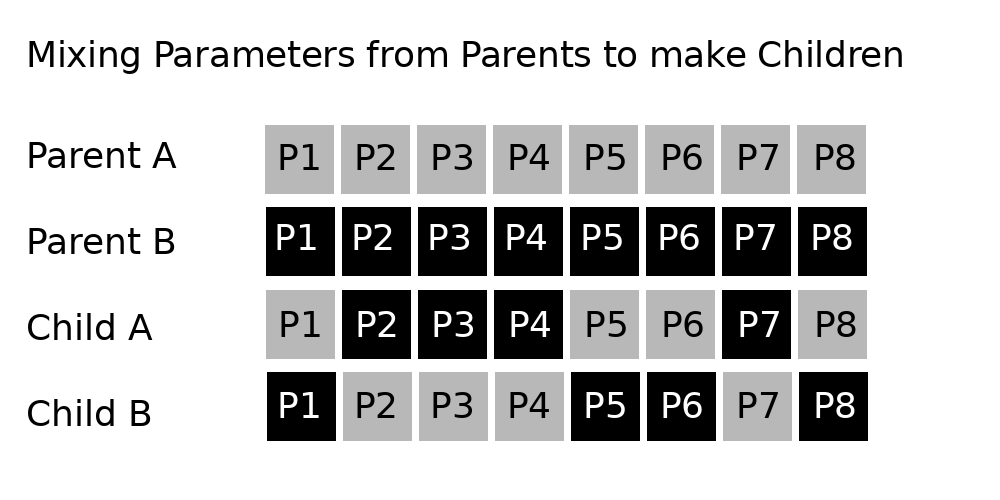
\includegraphics[scale=0.30]{chapters/potentials_fe_pd_ru/images/breeding.png}
    \caption{Parameter Breed Event}
    \label{fig:gabreedevent}
  \end{center}
\end{figure}

There is a chance that the child solutions will mutate slightly from the two parent combination, and this chance is set by the user.

During the breed event, the program will check whether or not the two children already exist within the solution pool.  If they are allowed to also enter the pool, the solutions may quickly be filled with clones during the breeding process.  The breed event automatically forces any clones to be varied so they become a different and distinct solution.

Every now and then an extinction event will occur that kills off any poor solutions and replaces them with variations of the better solutions.  The user controls the frequency of the extinction event and the probability that a solution will be removed.

Top solutions are enhanced, at a frequency picked by the user, using a local optimisation algorithm: line-search and gradient descent.  It does require many calculations and adds a substantial amount of time to the procedure, but it uses the gradient of solutions to find more optimal solutions more efficiently that randomly generated or bred solutions.

The algorithm used is given in the appendix (section \ref{section:geneticalgorithm}).


\subsubsection{Newton Gauss Optimisation}

The Newton Gauss optimisation estimates the second order derivatives matrix, the Hessian, by multiplying the Jacobian and its transpose.  It is not yet implemented in the code, but may be in the future.  The algorithm is used to find a local optimum, but it can be unstable or return errors.

\begin{equation}
\begin{split}
\vec{J}^{T} \vec{J} \vec{p} = \vec{J}^{T} \vec{r} \\
\vec{r} = \vec{y} - f(\vec{x}, \vec{p})
\end{split}
\label{eq:eqNewtonGauss}
\end{equation}

\subsubsection{Levenberg-Marquardt Optimisation}

The Levenberg-Marquardt algorithm is similar to the Newton-Gauss method, but the estimate for the Hessian does not need to be calculated for each loop of the algorithm.  The parameter, $\lambda$, is changed and the Hessian is updated periodically.  This is not yet implemented in the code, but may be added in the future.

\begin{equation}
\begin{split}
\left( \vec{J}^{T} \vec{W} \vec{J} + \lambda diag\left( \vec{J}^{T} \vec{W} \vec{J} \right) \right) \vec{p} = {\left(\vec{J}^{T} \vec{W} \vec{r} \right)} \\
\vec{r} = \vec{y} - f(\vec{x}, \vec{p})
\end{split}
\label{eq:eqLevenbergMarquardt}
\end{equation}


\subsubsection{Python SciPy Optimization Functions}

Additional optimisation functions have been used by importing the SciPy module into the program, and these may be used in conjunction with those listed above.  Several have been used including the bin-hopping, Nealder-Meade and \acrshort{bfgs}.  The bin-hopping was unreliable and crashed on a number of occasions, so I used the simulated annealing and genetic algorithms programmed specifically for this work.  The Nealder-Meade and \acrshort{bfgs} were both used following the run of global optimisation and increased the efficiency of improving the parameters.








\subsubsection{Minimising Runtime}











When fitting a potential, for each trial set of functions, the program must calculate the energy, forces and stress for each of the configurations and tens or hundreds of energy only calculations for the equation of state and elastic constant calculations.  Python is a well used programming language in many areas of Science and it has the benefits of many modern languages.  For certain specific tasks, it is slow in comparison to Fortran.

The energy, stress and force calculations were programmed in Fortran and use OpenMP to calculate the many configurations in parallel.  On a single thread, the fitting process could take weeks, but on a 20 core node the calculation time was reduced to under a couple of days.

not relevant

The first version of the code used tabulated potentials, and this removed the task of programming different functions (and the wide range of complexities amongst those functions) and replaced it with a quick search and interpolation of tabulated data.  However, the final version was developed to use and fit with analytic potentials.  Several of the optional functions, including the knot-to-knot spline function, drastically increased the computational time.  

The bulk property module in particular uses configurations with atoms in regular places, with there being a small set of unique atom separation values.  Rather than generate tabulated data for each function, to then interpolate, the input and output values are cached.  Once the value is calculated, it is quickly retrieved for subsequent calculations with the same input value.  The has increased computation speed of the analytic potentials to a speed similar to using tabulated functions.

In the current version, only analytic potentials are available for fitting.  There are several subroutines ready if tabulated functions are reintroduced.  These subroutines use Lagrange polynomials to interpolate values of the function (eq. \ref{eq:eqLagrangeDataSet} \ref{eq:eqLagrangePolynomialNew}).

\begin{equation}
\begin{split}
D = \lbrace \left(x_0, y_0 \right) \left(x_1, y_1 \right) \left(x_2, y_2 \right) \dotsm \left(x_n, y_n \right) \rbrace
\end{split}
\label{eq:eqLagrangeDataSet}
\end{equation}

\begin{equation}
\begin{split}
p_n (x) = \sum _{i=0} ^n y_i L(i, x) 
\textnormal{where    } l(i, x) = \prod _{j=0 , j!=i} ^n (x - x_j)
\end{split}
\label{eq:eqLagrangePolynomialNew}
\end{equation}

There are typically hundreds or thousands of data points, so to interpolate, the closest few points are used.  Throughout the computer code four point interpolation was the preferred method, to balance computational speed with a well fitting polynomial.  

The gradient of the potential functions are also computed using Lagrange polynomials (eq. \ref{eq:eqLagrangePolynomialNew}).

%% Sample hybrid function
\begin{equation}
\begin{split}
q_n \left( x \right) = \sum_{i=0}^{i=n} y_{i} g \left(i,  x \right) \\
\textnormal{where    } g \left(i, x \right) = \left( \prod_{j=0, j \neq i}^{j=n} \frac{1}{x_i - x_j} \right) \times \left( \sum_{k=0, k \neq i}^{k=n} \prod_{j=0, j \neq k, j \neq i}^{j=n} \left( x - x_j \right) \right)
\end{split}
\label{eq:eqLagrangePolynomialNew}
\end{equation}

A pseudocode for both interpolation of the function points and derivatives are available in the appendix (section \ref{section:interpolationpseudo} and \ref{section:interpolationgradientpseudo}).



\subsubsection{Effective Gauge Transforms}

In order to create a potential for an alloy an effective gauge transform, as described in section \ref{section:pairembeddingsym}, was applied to each pure potential.  A mode added to the EAMPA program reads in the analytic potential and creates a numeric potential that has had the transform applied.  This allows the pure potentials to be used together, although a cross pair potential is still needed.



\subsubsection{LAMMPS Format}






\subsection{Verifying Energy and Force Calculations with LAMMPS}

Many of the calculations depend on the energies computed as well as accurate computation of the forces.  \acrshort{lammps} is a widely used molecular dynamics code and many potentials already exists in the format required for \acrshort{lammps}.



